\subsection{Materials Project}
{{\footnotesize
\noindent The Materials Project provides an open-access database of computed properties for
inorganic materials via high-throughput density functional theory (DFT), accelerating 
materials discovery.


\begin{description}[labelwidth=4cm, labelsep=1em, leftmargin=4cm, itemsep=0.1em, parsep=0em]
  \item[date:] 2011-10-01
  \item[version:] 1
  \item[last\_updated:] 2011-10-01
  \item[expired:] false
  \item[valid:] yes
  \item[valid\_date:] 2011-10-01
  \item[url:] \href{https://materialsproject.org/}{https://materialsproject.org/}
  \item[doi:] unknown
  \item[domain:] Materials Science
  \item[focus:] DFT-based property prediction
  \item[keywords:]
    - DFT
    - materials genome
    - high-throughput
  \item[licensing:] https://next-gen.materialsproject.org/about/terms
  \item[task\_types:]
    - Property prediction
  \item[ai\_capability\_measured:]
    - Prediction of inorganic material properties
  \item[metrics:]
    - MAE
    - R\textasciicircum{}2
  \item[models:]
    - Automatminer
    - Crystal Graph Neural Networks
  \item[ml\_motif:]
    - Material properties
  \item[type:] Benchmark
  \item[ml\_task:]
    - Supervised Learning
  \item[solutions:] 0
  \item[notes:] Core component of the Materials Genome Initiative
  \item[contact.name:] unknown
  \item[contact.email:] unknown
  \item[datasets.links.name:] Materials Project Catalysis Explorer
  \item[datasets.links.url:] \href{https://next-gen.materialsproject.org/catalysis}{https://next-gen.materialsproject.org/catalysis}
  \item[results.links.name:] unknown
  \item[results.links.url:] \href{unknown}{unknown}
  \item[fair.reproducible:] True
  \item[fair.benchmark\_ready:] True
  \item[id:] materials\_project
  \item[Citations:] \cite{jain2013materials}
\end{description}

{\bf Ratings:} ~ \\

\begin{tabular}{p{0.15\textwidth} p{0.07\textwidth} p{0.7\textwidth}}
\hline
Rating & Value & Reason \\
\hline
dataset & 3 & API key required to access data. No predefined splits.
 \\
documentation & 0 & No explanations or paper provided
 \\
metrics & 5 & Uses numerical metrics like MAE and R^2
 \\
reference\_solution & 2 & Numerous models (e.g., Automatminer, CGCNN) trained on the database, but no constraints or documentation listed.
 \\
software & 0 & No instructions available
 \\
specification & 1.5 & The platform offers a wide range of material property prediction tasks, but task framing and I/O formats vary by API use and are not always standardized across use cases.
 \\
\hline
\end{tabular}

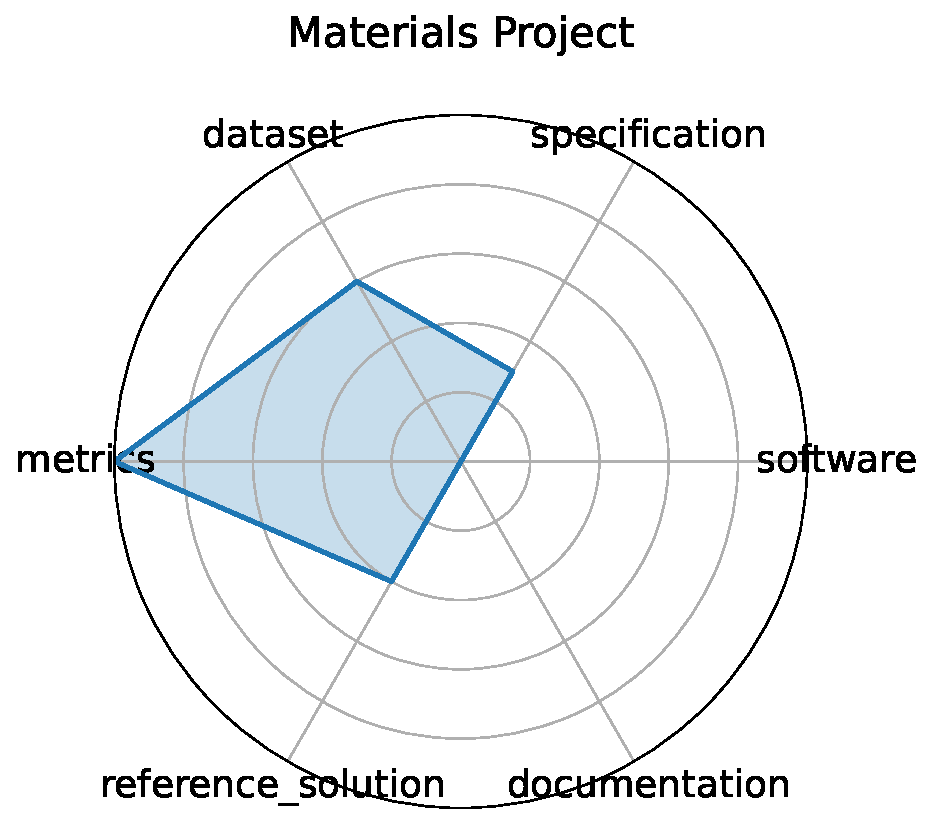
\includegraphics[width=0.2\textwidth]{materials_project_radar.pdf}
}}
\clearpage